\chapter{基础理论}
多目标跟踪技术在智能感知与视觉理解等领域具有重要应用价值,其核心难点在于复杂场景下的轨迹关联与身份保持。
为更好地理解本文后续提出的多目标跟踪与跨域自适应方法,本章对相关基础理论进行介绍。首先阐述图的基本概念及图神经网络的核心原理,
为基于图结构的轨迹关联方法提供理论支撑;随后介绍跨域视觉感知与自适应建模的基本思想,
分析恶劣视觉条件引起的域偏移问题;最后给出本文实验中使用的数据集与评价指标。
\section{图神经网络相关理论及方法}
图神经网络是一类能够直接作用于图结构数据的深度学习模型,在建模非结构化数据及复杂关系方面具有显著优势。
鉴于多目标跟踪中的轨迹关联问题天然具备图结构特性,引入图神经网络为刻画目标之间的关联关系提供了有效工具。
为系统介绍图神经网络的相关理论,本节首先从图的基本概念出发,阐述节点、边及其特征的表示方式,
并简要介绍图神经网络在不同层级任务中的应用。
随后,对图神经网络的谱域与空域方法进行分类说明,重点介绍基于消息传递机制的空域建模方法。
\subsection{图神经网络基本理论及应用}
\textbf{1. 图基本概念}

图(Graph)是一种用于描述对象及其交互关系的基本数据结构,广泛应用于具有复杂关系的非结构化数据。
假设一个图$G$包含$M$个节点和$N$条边,节点集合用$V=\{v_1,v_2,\cdots,v_M\}$表示,每个节点$v_i$可以表示成一个实体(如视频帧中的一个检测目标)。
边集合$E$用于描述节点之间的连接关系,定义为$E=\lbrace e_{i,j} = (v_i,v_j) ~ |~ v_i,v_j\in V,\quad |E|=N \rbrace$,
其中$e_{i,j}$表示从节点$v_i$指向节点$v_j$的一条边。
在无向图中,$e_{i,j}$与$e_{j,i}$表示同一条边;而在有向图中,$e_{i,j}$与$e_{j,i}$表示两条方向相反、相互独立的有向边。
综上,图$G$可形式化表示为$G=(V,E)$,由节点集合和边集合共同构成。

在实际计算中,图的连接关系通常采用邻接表(Adjacency List)等稀疏数据结构进行存储,以提升在大规模图上的计算与存储效率。
对于无向图,每一条边需要在相邻两个节点的邻接表中分别存储一次;而对于有向图,每条边仅需存储一次。
因此,在采用邻接表表示的情况下,无向图在存储开销上通常是对应有向图的两倍(假设边数量相同)。

除了结构信息外,图通常还具备丰富的特征信息。节点属性矩阵一般表示为$X_v\in \mathbb{R}^{M\times C_v}$,其中$C_v$是每个节点的特征数,可包含外观、运动、空间位置等属性;
边属性矩阵则表示为$X_e \in \mathbb{R}^{N\times C_e}$,其中$C_e$是每条边的特征数,用于刻画节点之间的关系属性,如相对位移、时序间隔、相似度度量或关系类型等。

图神经网络的目标是通过结合图结构信息和节点、边属性,学习到更高级的节点嵌入(节点$v_i$的嵌入表示为$h_i$)和边嵌入(边$e_{i,j}$的嵌入表示为$z_{i,j}$),
从而支撑各类图分析任务。

\autoref{tab:ch2_1}给出了本文图神经网络建模中涉及的主要概念及其对应符号。

\begin{table}[htbp]
    \caption{\label{tab:ch2_1}图神经网络建模中主要概念及其对应符号}
    \begin{tabularx}{\linewidth}{c|X<{\centering}}
        \hline
        \textbf{概念} & \textbf{符号} \\ \hline
        节点数量 & $M$ \\ \hline
        节点集合 & $V=\{v_1,v_2,\cdots,v_M\}$ \\ \hline
        边数量 & $N$ \\ \hline
        边集合 & $E=\lbrace e_{i,j} = (v_i,v_j) ~ |~ v_i,v_j\in V,\ |E|=N \rbrace$ \\ \hline
        图 & $G=(V,E)$ \\ \hline
        节点属性矩阵 & $X_v \in \mathbb{R}^{M\times C_v}$ \\ \hline
        边属性矩阵 & $X_e \in \mathbb{R}^{N\times C_e}$ \\ \hline
        节点$v_i$的节点嵌入 & $h_i$ \\ \hline
        节点$v_i$与$v_j$之间的边嵌入 & $z_{i,j}$ \\ \hline
    \end{tabularx}
\end{table}

\textbf{2. 图神经网络应用}

根据任务目标的粒度,图神经网络的应用可归纳为图层级(Graph-level Tasks)、边层级(Edge-level Tasks)和节点层级(Node-level Tasks)三类任务,
不同层级对应着不同粒度的图元素分类或回归的需求。
\begin{itemize}
    \item 图层级任务主要关注图的整体结构信息,如图的分类、聚类、分割等。例如,在社交网络分析中,图层级任务可应用于社区发现,通过分析节点间的连接关系,识别出具有相似特征或紧密关系的节点群体。
    \item 边层级任务以图中的边为预测对象,关注节点之间关系的判别或数值估计。例如,在推荐系统中,边层级任务可应用于预测用户之间的交互关系,通过分析用户之间的连接关系,预测用户是否会相互交互。
    \item 节点层级任务则以节点为基本预测单元,目标是对节点状态或属性进行分类或回归建模。该类方法通过聚合节点邻域信息,结合节点自身特征,学习具有判别能力的节点表示,从而完成节点级预测。
例如,在知识图谱中,点层级任务可应用于实体分类,通过分析实体之间的连接关系,识别出实体的类别。
\end{itemize}

在\ref{subsec:gnn_apply}小节中提及到的图跟踪算法(如GCNNMatch\cite{gcnnmatch}、MPNTracker\cite{MPNTracker}等)大多将轨迹关联问题建模为边层级的二分类任务,并基于无向图构建全连接图结构。
然而,这类方法需要对海量侯选边进行打分和筛选,计算复杂且易受噪声干扰。与这些方法不同的是,本文第三章提出的双图协同关联框架,在本质上将轨迹关联
问题创新性地定义成一个节点层级的分类任务,并基于有向图建模,从而提升了算法的效率与跟踪性能。

\subsection{图神经网络的谱域与空域方法}

图神经网络通过对节点及其邻域信息的迭代聚合与变换来学习有效的图表示。根据其理论基础与实现机制,主要可分为基于谱图理论(谱域)的方法和基于空间关系(空域)的方法两大类。

\textbf{1. 谱域方法:基于谱图理论的卷积}

2013年,Bruna等人\cite{bruna}首次将谱图理论与卷积神经网络相结合,其核心思想是借助图傅里叶变换(Graph Fourier Transform),将定义在图节点上的信号$X_v$(即节点属性矩阵)转换到
由拉普拉斯矩阵特征向量张成的谱域中进行滤波,
再逆变换回空域,从而在图结构上模拟了卷积过程。谱域图卷积操作可形式化表示为:
\begin{equation}
Y_v = U g_\theta(\Lambda) U^T X_v
\label{equ:gcn_1}
\end{equation}
其中,$X_v$是输入节点信号,$Y_v$是卷积后的输出信号;$U$是图傅里叶矩阵,$\Lambda$是图傅里叶矩阵对应的频率对角矩阵;$g_\theta(\Lambda)=diag(\theta)$是一个可学习的对角矩阵,
代表作用于不同频率分量的谱滤波器。

但是,由\autoref{equ:gcn_1}定义的图卷积操作需要显式计算拉普拉斯矩阵的特征分解,其时间复杂度较高(约为 $\mathcal{O}(M^2)$),同时滤波器依赖于全局图结构,难以在大规模或结构变化的图上高效拓展。为提升效率,后续工作采用了多项式滤波器进行逼近,如切比雪夫多项式(ChebNet\cite{defferrard}),
进一步对图卷积进行了简化,使其能够在实际任务中高效训练。

尽管谱域方法具有坚实的数学理论基础,能清晰地刻画信号在图上的平滑性与频率响应,但其仍存在一定局限性:其一,谱域卷积依赖于特定图结构的拉普拉斯特征分解,难以直接迁移到结构变化的图上;
其二,谱域方法通常假设图为无向且静态,这在动态图或有向图建模中具有一定限制。
因此,在需要处理动态图结构或复杂关系建模的应用场景中,谱域方法的适用性受到一定约束。

\textbf{2. 空域方法:基于消息传递的范式}

与依赖全局谱变换的谱域方法不同,空域图神经网络方法直接在图结构的空间域上定义信息传播与特征更新规则,通过刻画节点与其邻居之间的局部交互关系来学习图表示。
目前,消息传递神经网络(Message Passing Neural Network,MPNN)\cite{mpnn}因其形式统一、表达灵活,已成为空域图神经网络的主流范式之一。

MPNN 的核心思想是通过迭代的消息传递过程,使图中每个节点能够逐步融合来自邻域的结构与特征信息。
如\autoref{fig:ch2_1}所示,以第 $l$ 层消息传递层为例,MPNN 通常通过消息构建、消息聚合和节点更新三个步骤,对节点表示完成一次迭代更新。
\begin{figure}[htbp]
    \centering
    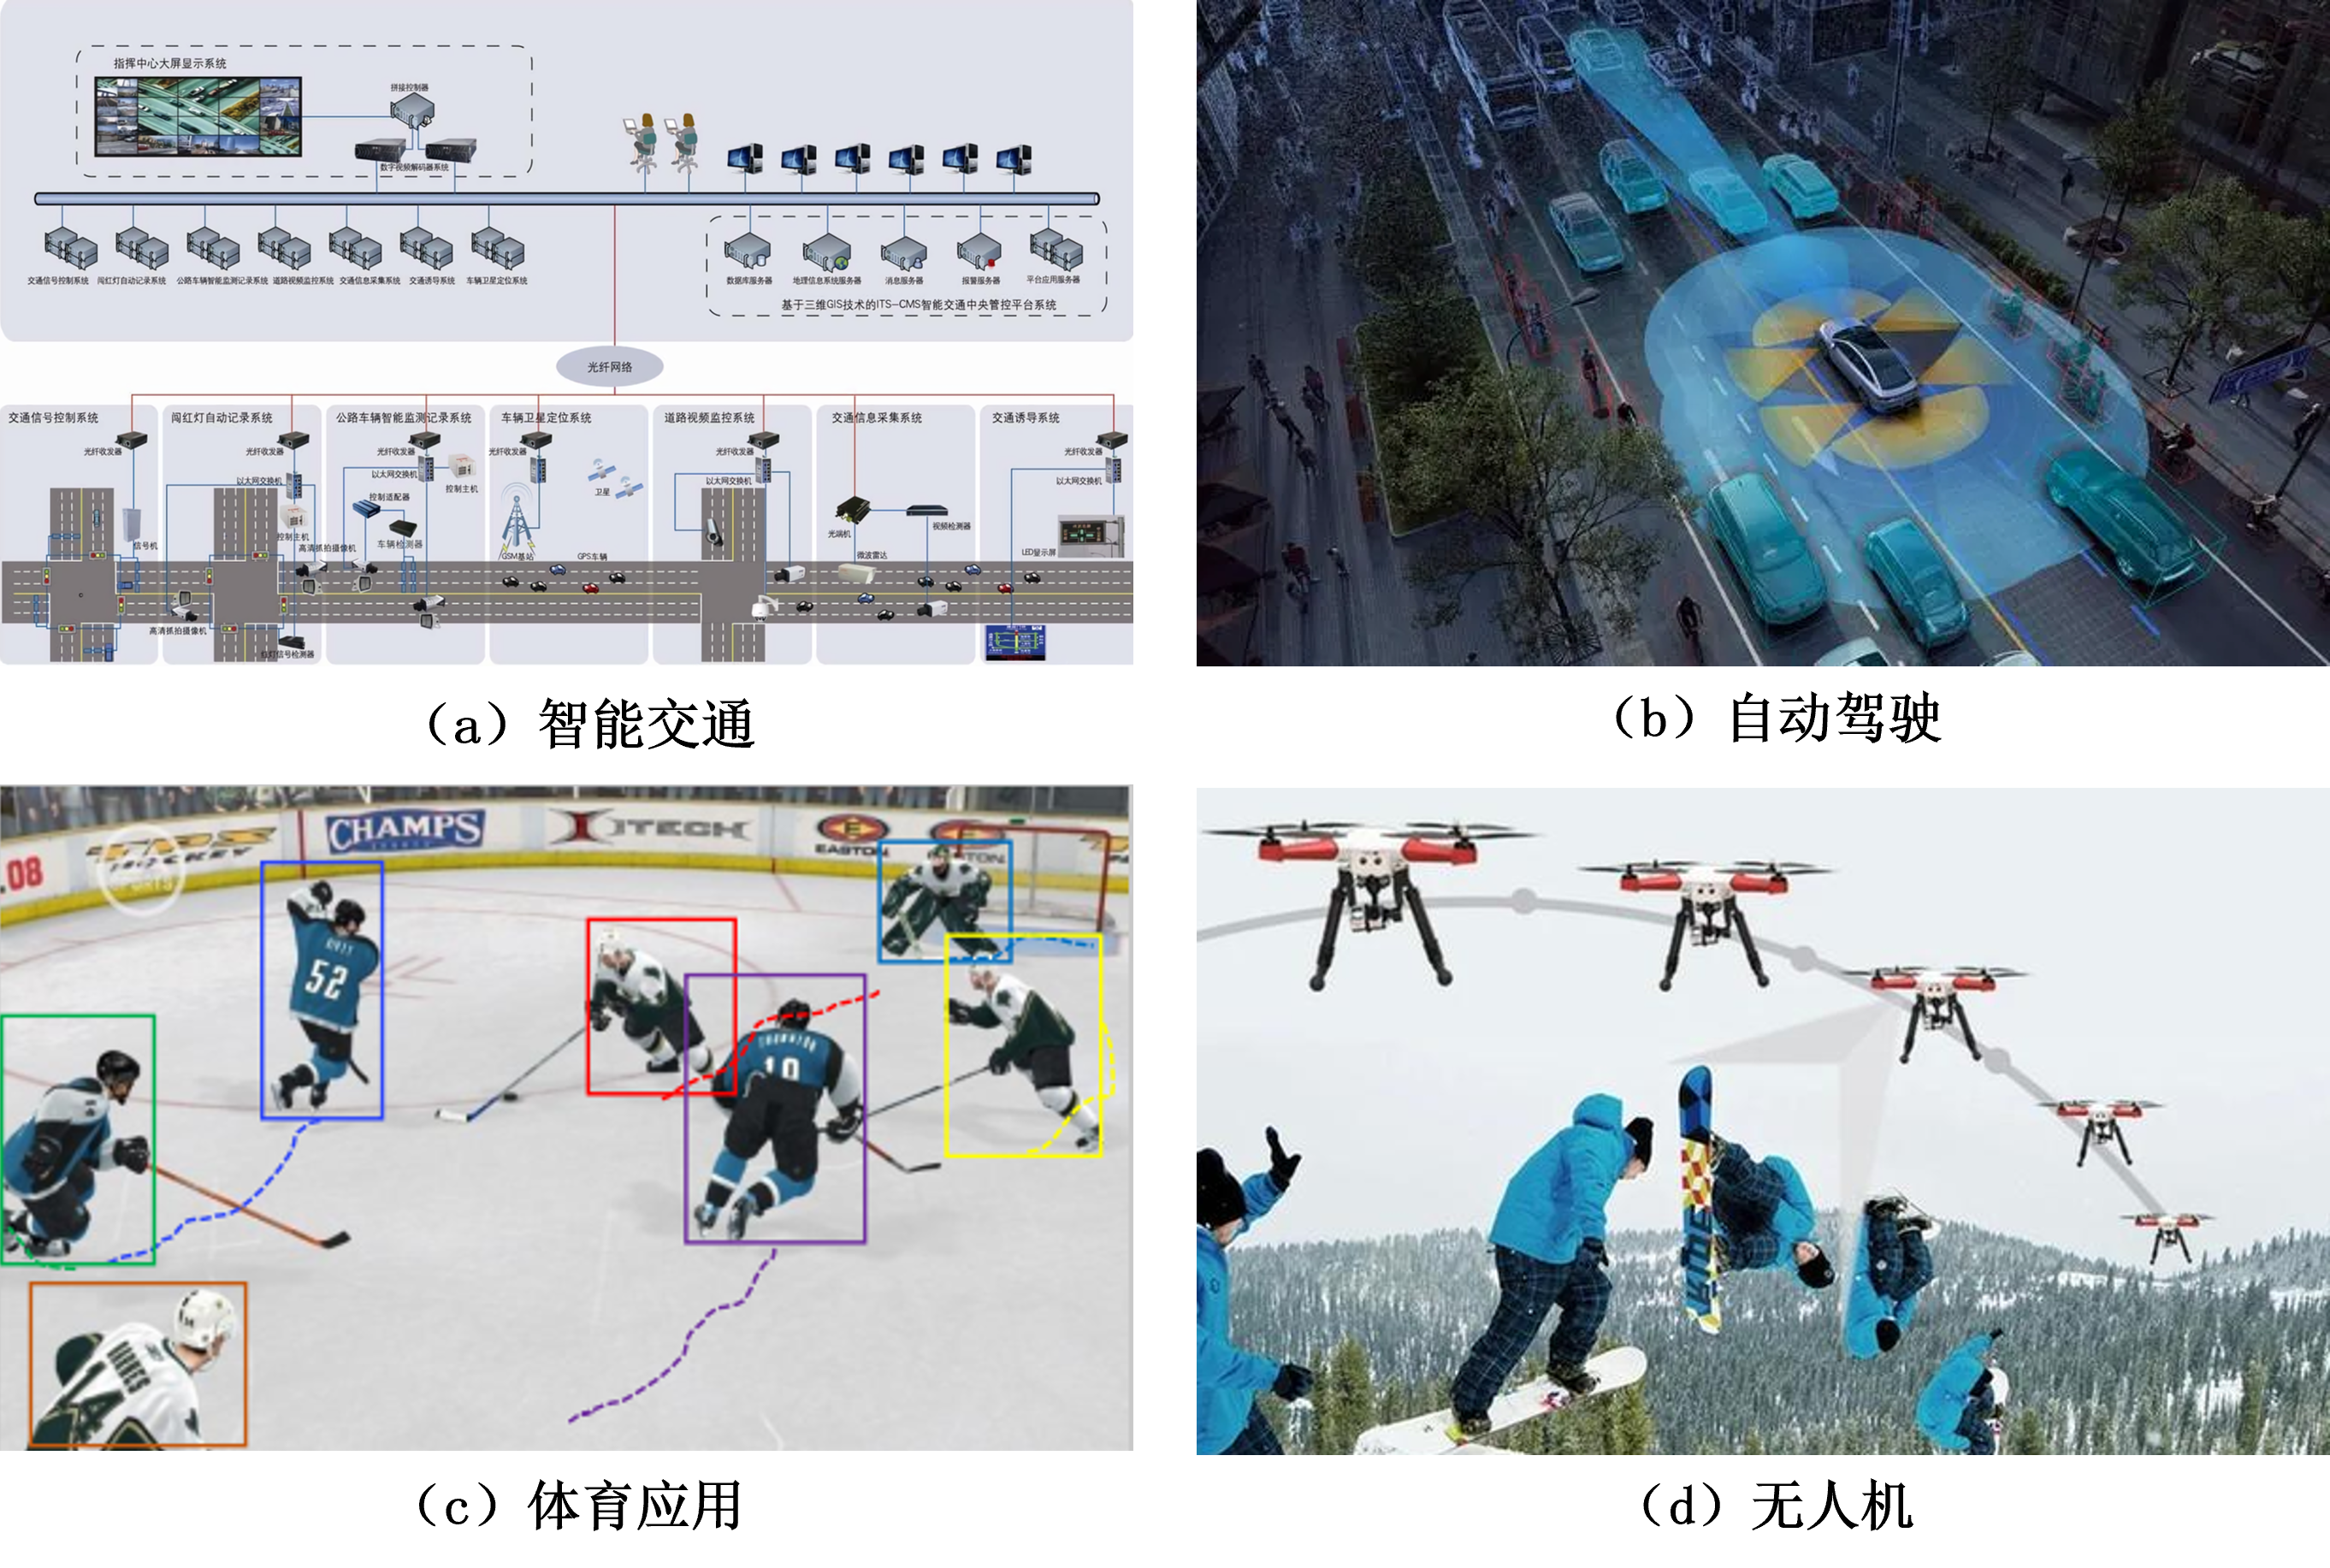
\includegraphics[width=15cm]{chapter2/1.png}
    \caption{\label{fig:ch2_1}基于消息传递的图神经网络更新流程}
\end{figure}


\textbf{1. 消息构建}。对于图中的每一条有向边 $e_{ji}$(从源节点 $v_j$ 指向目标节点 $v_i$),生成一条传递消息。
该消息由源节点 $
v_j$ 的当前嵌入 $h_j^{(l)}$、目标节点 $v_i$ 的当前嵌入 $h_i^{(l)}$以及对应的边嵌入 $z_{j,i}^{(l)}$ 共同决定:
\begin{equation}
    m_{ji}^{(l)}=\text{MESSAGE}^{(l)}\left(h_j^{(l)}, h_i^{(l)}, z_{j,i}^{(l)}\right)
    \label{equ:msg}
\end{equation}
其中,$\text{MESSAGE}^{(l)}(\cdot)$ 为可微消息函数,通常由多层感知机(Multilayer Perceptron,MLP)实现。

\textbf{2. 消息聚合}。对于每个目标节点 $v_i$,将其所有来自邻域 $\mathcal{N}_i$ 的消息进行聚合:
\begin{equation}
    M_i^{(l)}=\text{AGGREGATE}^{(l)}\left(\{m_{ji}^{(l)} \mid j \in \mathcal{N}_i\}\right)
    \label{equ:agg}
\end{equation}
其中,$\text{AGGREGATE}^{(l)}(\cdot)$ 为聚合函数,常见形式包括求和、求平均或取最值等具有排列不变性的操作。

\textbf{3. 节点更新}。每个目标节点 $v_i$ 结合自身上一层的节点嵌入 $h_i^{(l)}$与聚合后的邻域信息 $M_i^{(l)}$,更新其节点表示:
\begin{equation}
    h_i^{(l+1)}=\text{UPDATE}^{(l)}\left(h_i^{(l)}, M_i^{(l)}\right)
    \label{equ:update}
\end{equation}
其中,$\text{UPDATE}^{(l)}(\cdot)$ 为节点更新函数,同样可以采用 MLP 等可学习模块实现。

通过堆叠 $L$ 层这样的消息传递层,节点 $v_i$ 的表示能够逐步融合其 $L$ 跳邻域内的信息,从而实现对更大范围结构关系的建模。

综上所述,与谱域方法相比,空域图神经网络不依赖于固定图结构的谱信息,因而在动态图建模、异构关系刻画以及有向图场景中具有更强的灵活性和可拓展性。
本文第三章的方法采用该消息传递范式进行建模与实现。

\section{跨域视觉感知与自适应建模基础}

\section{数据集与评价方法}

\section{本章小结}